\documentclass[a4paper]{scrartcl}
\usepackage{scrpage2}
\usepackage[ngerman]{babel}
\usepackage[T1]{fontenc}
\usepackage[utf8]{inputenc}
%\usepackage[pdftex]{graphicx}
%\usepackage[intlimits]{amsmath}
%\usepackage{listings}
%\lstset{frame=single,breaklines=true}
\usepackage{ amssymb }
\usepackage{amsmath}
\usepackage{hyperref}
\usepackage{enumerate}
\usepackage[a4paper, total={19cm, 23cm}]{geometry}
\usepackage{stmaryrd}
\usepackage{graphicx}
\pagestyle{scrheadings}
\pagenumbering{gobble}
\ihead{Übungsblatt 3\\Nils Werner 108012219293}
\chead{\\Paul Rösler 108012225686	}
\ohead{Übungsgruppe: Mo. 16:00\\Daniel Teuchert 108012214552}
\setheadsepline{0.4pt}
\begin{document}

\section*{Aufgabe 1}
Zu zeigen: $\{nor, c\}$ ist universell, zeige: $nand$ kann durch $nor$ dargestellt werden, da $\{nand,c\}$ universell ist (siehe Vorlesung), ist dann auch $\{nor, c\}$ universell.

\begin{figure}[htp] \centering{
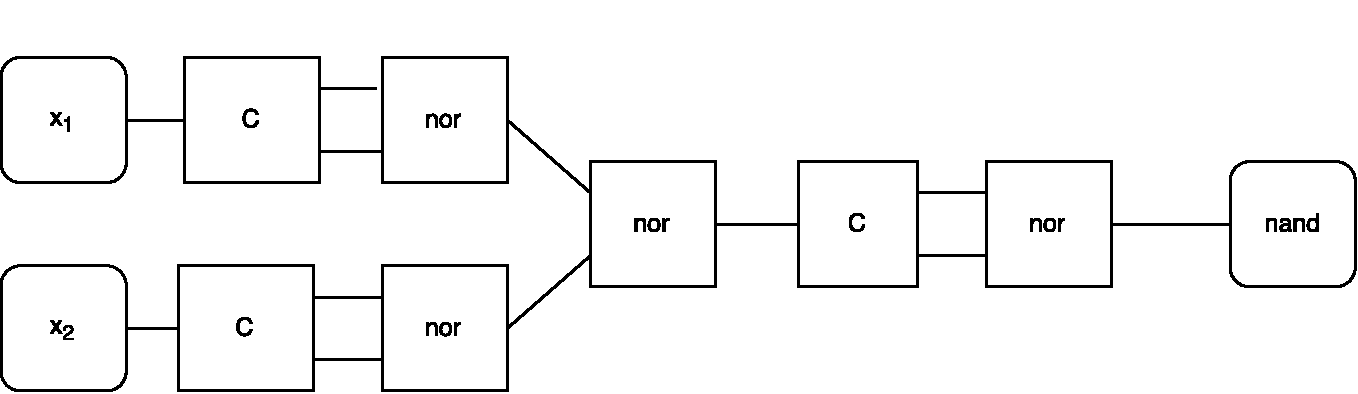
\includegraphics[scale=0.5]{nand.pdf}}
\caption{Schaltkreis $nand$ aus $nor$}
\end{figure}

$nand = \overline{\overline{\overline{x_1 \vee x_1} \vee \overline{x_2 \vee x_2}}~~\vee ~~\overline{\overline{x_1 \vee x_1} \vee \overline{x_2 \vee x_2}}}$\\
$= \overline{\overline{\overline{x_1} \vee \overline{x_2}}~~\vee ~~\overline{\overline{x_1} \vee \overline{x_2}}}$\\
$= \overline{(x_1 \wedge x_2)~~\vee ~~(x_1 \wedge x_2)}$\\
$= \overline{x_1 \wedge x_2}~~\wedge ~~\overline{x_1 \wedge x_2}$\\
$= \overline{x_1 \wedge x_2} = nand(x_1,x_2)$

\newpage
\section*{Aufgabe 2}

\begin{figure}[htp] \centering{
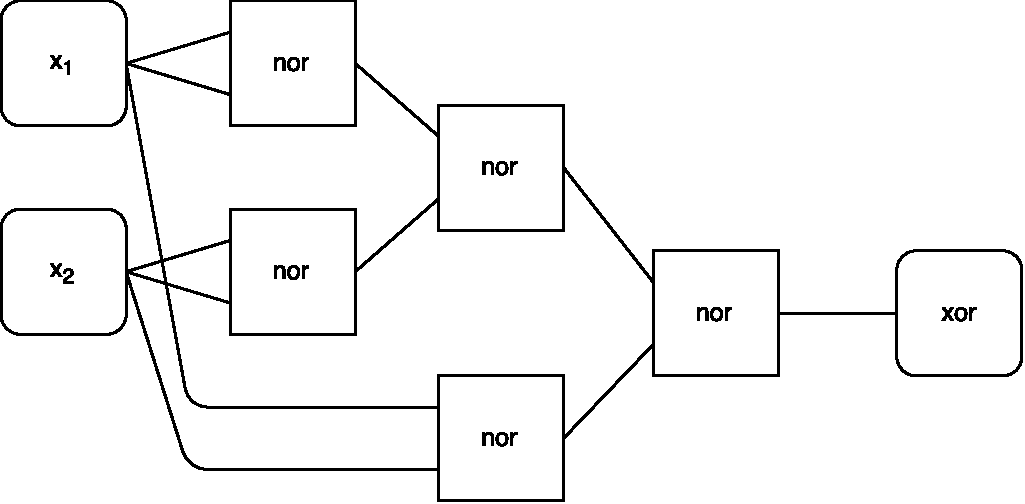
\includegraphics[scale=0.5]{xor.pdf}}
\caption{Schaltkreis $xor$ aus $nor$}
\end{figure}

\newpage
\section*{Aufgabe 3}

Beschreibung einer Funktion $f: \{0,1\}^n \rightarrow \{0,1\}^m$ als $f((x_1,...,x_n))=(y_1,...,y_m)$ mit Disjunktiver Normalform:\\
$y_j = ((\neg) x_1 \wedge (\neg) x_2 \wedge ... \wedge (\neg) x_n ) \vee ... \vee ((\neg) x_1 \wedge (\neg) x_2 \wedge ... \wedge (\neg) x_n )$ mit $1\leq j \leq m$ und $(\neg)$ symbolisiert eine mögliche Negierung.\\
Der Term $((\neg) x_1 \wedge (\neg) x_2 \wedge ... \wedge (\neg) x_n )$ existiert maximal $\lfloor n/2 \rfloor$ Mal in einer Gleichung, sonst wird die Konjunktive Normalform verwendet, die dann maximal $\lfloor n/2 \rfloor$ Terme mit $n$ Variablen enthält.\\
Unter der Annahme, dass die Operationen nur zwei Eingänge haben, sieht die Gleichung für jedes $y_j$ unter Verwendung der Disjunktiven Normalform wie folgt aus:
\begin{figure}[htp] \centering{
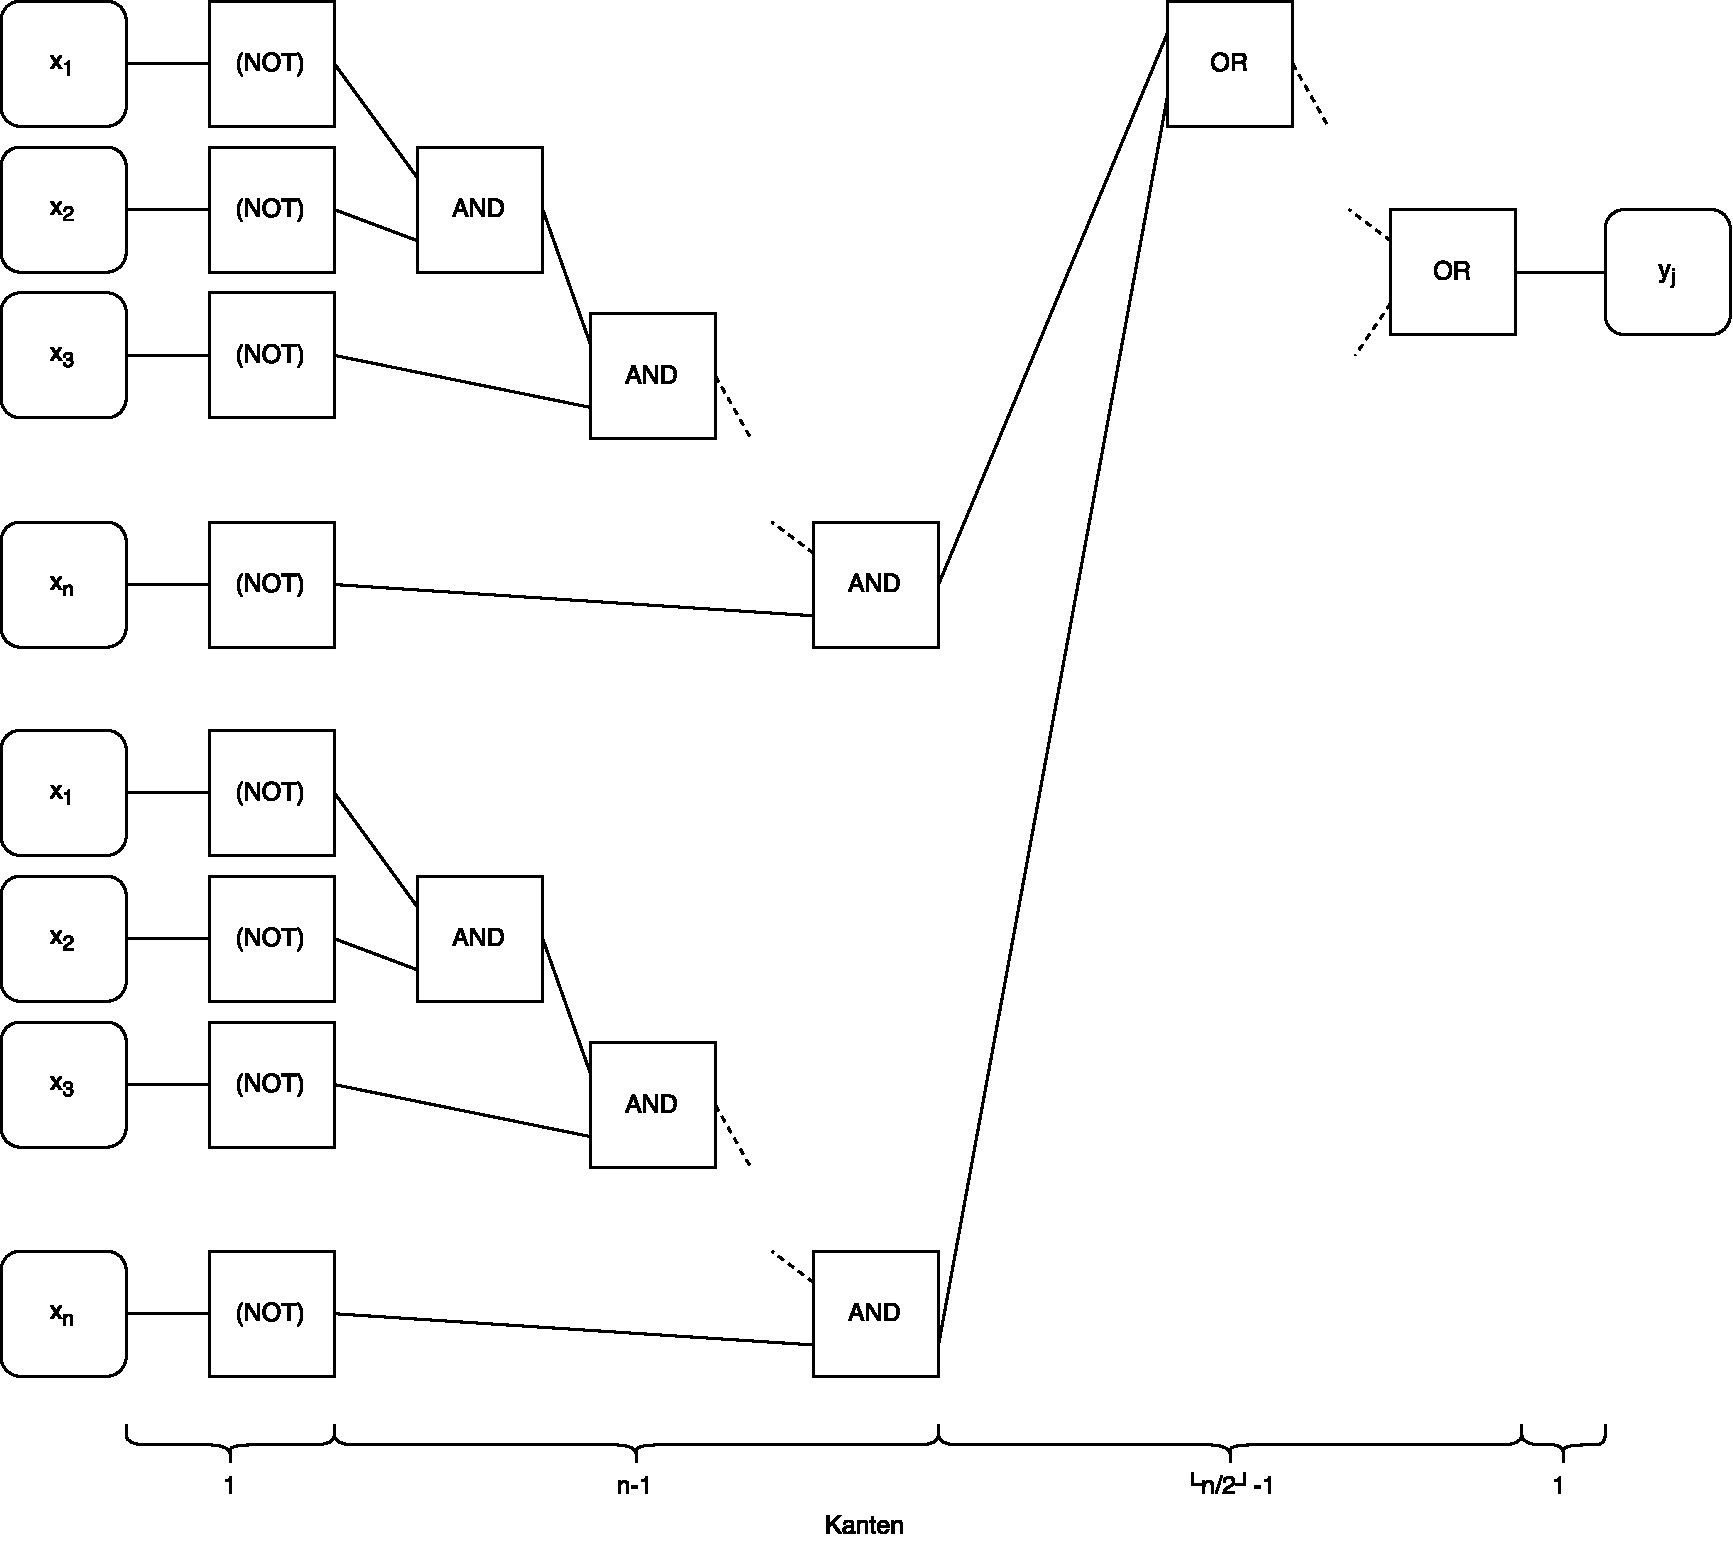
\includegraphics[scale=0.5]{dnf.pdf}}
\caption{Disjunktive Normalform für Funkion $f((x_1,...,x_n))=(y_1,...,y_m)$}
\end{figure}

Die Tiefe für $y_j$ ergibt der Weg zu $x_1$. Zwischen $x_1$ und $y_j$ befinden sich maxmial eine Negierung, $n-1~AND$ und $\lfloor n/2\rfloor -1~OR$ Operationen. Da die Schaltkreise für alle anderen $y_k$ mit $1\leq k\leq m \wedge j\neq k$ parallel zu dem Schaltkreis für $y_j$ verlaufen und das gleiche Maximum besitzen, hat der Weg zwischen einem Eingabeknoten und einem Ausgabeknoten in dieser Darstellung einer Funktion $f$ die maximale Länge $1+(n-1)+(\lfloor n/2\rfloor -1)+1$\\ $\leq \frac{3}{2} n \in O(n)$.\\
Da jede Funktion in der Disjunktiven bzw. Konjunktiven Normalform beschrieben werden kann und die Anzahl der Ausgabebits $m$ keinen Einfluss auf die Tiefe des Schaltkreises hat, gilt die Tiefe entsprechend für alle Funktionen $f: \{0,1\}^n \rightarrow \{0,1\}^m$.

\newpage
\section*{Aufgabe 4}
\begin{enumerate}[a)]

\item $M_C^{|a\rangle}(|b\rangle)$ ist der Erwartungswert des Zustands nach der Messung durch $C$ in der Basis mit $|a\rangle$ von $|b\rangle$.\\
$|y\rangle = \frac{1}{\sqrt{2}} (|0\rangle -|1\rangle)$

$P[b=0] = P[M_B^{|0\rangle}(|z'\rangle)=|0\rangle~|~a'=0]~P[a'=0] + P[M_B^{|x\rangle}(|z'\rangle)=|x\rangle~|~a'=1]~P[a'=1]$\\
$=P[M_B^{|0\rangle}(M_E^{|\alpha \rangle}(|z\rangle))=|0\rangle~|~a'=0]~\frac{1}{2} + P[M_B^{|x\rangle}(M_E^{|\alpha \rangle}(|z\rangle))=|x\rangle~|~a'=1]~\frac{1}{2}$\\
$=\frac{1}{2} (P[M_B^{|0\rangle}(M_E^{|\alpha \rangle}(|0\rangle))=|0\rangle~|~a'=0 \wedge a=0]~P[a=0] + P[M_B^{|0\rangle}(M_E^{|\alpha \rangle}(|x\rangle))=|0\rangle~|~a'=0 \wedge a=1]~P[a=1])$\\
$+\frac{1}{2} (P[M_B^{|x\rangle}(M_E^{|\alpha \rangle}(|0\rangle))=|x\rangle~|~a'=1 \wedge a=0]~P[a=0] + P[M_B^{|x\rangle}(M_E^{|\alpha \rangle}(|x\rangle))=|x\rangle~|~a'=0 \wedge a=1]~P[a=1])$\\
$=\frac{1}{4} (P[M_B^{|0\rangle}(|\langle \alpha|0\rangle|~|\alpha\rangle + |\langle \beta|0\rangle|~|\beta\rangle)=|0\rangle] + P[M_B^{|0\rangle}(|\langle \alpha|x\rangle|~|\alpha\rangle + |\langle \beta|x\rangle|~|\beta\rangle)=|0\rangle]$\\
$+ P[M_B^{|x\rangle}(|\langle \alpha|0\rangle|~|\alpha\rangle + |\langle \beta|0\rangle|~|\beta\rangle)=|x\rangle] + P[M_B^{|x\rangle}(|\langle \alpha|x\rangle|~|\alpha\rangle + |\langle \beta|x\rangle|~|\beta\rangle)=|x\rangle])$\\
$=\frac{1}{4} (P[|\langle 0|(|\langle \alpha|0\rangle|~|\alpha\rangle + |\langle \beta|0\rangle|~|\beta\rangle)|~|0\rangle + |\langle 1|(|\langle \alpha|0\rangle|~|\alpha\rangle + |\langle \beta|0\rangle|~|\beta\rangle)|~|1\rangle=|0\rangle]$\\
$+ P[|\langle 0|(|\langle \alpha|x\rangle|~|\alpha\rangle + |\langle \beta|x\rangle|~|\beta\rangle)|~|0\rangle + |\langle 1|(|\langle \alpha|x\rangle|~|\alpha\rangle + |\langle \beta|x\rangle|~|\beta\rangle)|~|1\rangle =|0\rangle]$\\
$+ P[|\langle x| (|\langle \alpha|0\rangle|~|\alpha\rangle + |\langle \beta|0\rangle|~|\beta\rangle)|~|x\rangle + |\langle y| (|\langle \alpha|0\rangle|~|\alpha\rangle + |\langle \beta|0\rangle|~|\beta\rangle)|~|y\rangle =|x\rangle]$\\
$+ P[|\langle x| (|\langle \alpha|x\rangle|~|\alpha\rangle + |\langle \beta|x\rangle|~|\beta\rangle)|~|x\rangle + |\langle y| (|\langle \alpha|x\rangle|~|\alpha\rangle + |\langle \beta|x\rangle|~|\beta\rangle)|~|y\rangle =|x\rangle])$\\
$=\frac{1}{4} (P[(|\langle \alpha|0\rangle|^2 + |\langle \beta|0\rangle|^2)~|0\rangle + (|\langle \alpha|0\rangle|~|\langle \alpha|1\rangle| + |\langle \beta|0\rangle|~|\langle \beta|1\rangle|)~|1\rangle=|0\rangle]$\\\\
TODO: 
$+ P[|\langle 0|(|\langle \alpha|x\rangle|~|\alpha\rangle + |\langle \beta|x\rangle|~|\beta\rangle)|~|0\rangle + |\langle 1|(|\langle \alpha|x\rangle|~|\alpha\rangle + |\langle \beta|x\rangle|~|\beta\rangle)|~|1\rangle =|0\rangle]$\\
$+ P[|\langle x| (|\langle \alpha|0\rangle|~|\alpha\rangle + |\langle \beta|0\rangle|~|\beta\rangle)|~|x\rangle + |\langle y| (|\langle \alpha|0\rangle|~|\alpha\rangle + |\langle \beta|0\rangle|~|\beta\rangle)|~|y\rangle =|x\rangle]$\\
$+ P[|\langle x| (|\langle \alpha|x\rangle|~|\alpha\rangle + |\langle \beta|x\rangle|~|\beta\rangle)|~|x\rangle + |\langle y| (|\langle \alpha|x\rangle|~|\alpha\rangle + |\langle \beta|x\rangle|~|\beta\rangle)|~|y\rangle =|x\rangle])$\\



\end{enumerate}
\end{document}
